\documentclass[../main.tex]{subfiles}
\begin{document}
\subsection{Introduzione}
Una funzione $f$ è una legge che associa ad ogni elemento $x$ di un insieme di partenza $A$ un \textbf{unico} elemento $y$ di un insieme di arrivo $B$.
\begin{center}
    \begin{tikzpicture}
        %sets A and B
        \draw (0,0) ellipse (1 and 2);
        \draw (5,0) ellipse (1 and 2);
        \node at (0, 2.3) {$A$};
        \node at (5,2.3) {$B$};
        \node at (2.5,0.3) {$f$};
        
        %set A
        \node at (0,0) {$\bullet$};
        \node at (-0.2,0.2) {$x$};

        
        %set B
        \node at (5,0) {$\bullet$};
        \node at (5.2,0.2) {$y$};
        
        %arrows
        \draw[->] (0.2,0) -- (4.8,0);
    \end{tikzpicture}
    \begin{align*}
        f:A& \longrightarrow B \\
        x& \longmapsto y = f(x)
    \end{align*}
\end{center}
$x$ è detto elemento di $A$ associato a $y$, elemento di $B$. \\

\subsubsection{Esempi}
\begin{enumerate}
    \item \begin{align*}
        f: \mathbb{R}& \longrightarrow \mathbb{R} \\
        x& \longmapsto y=3x-2 \\
        x&=5 \Rightarrow y=3\cdot5-2=13 \\
        &\Rightarrow f \text{ è una funzione}
    \end{align*}
    \item \begin{align*}
        f: \mathbb{R}& \longrightarrow \mathbb{R} \\
        x& \longmapsto y=\sqrt{x} \\
        x&=4 \Rightarrow y=\sqrt{4}=2 \\
        x&=-4 \Rightarrow y=\sqrt{-4} \\
        &\sqrt{-4} \text{ non esiste in } \mathbb{R} \\
        &\Rightarrow f \text{ non è una funzione}
    \end{align*}
    \item \begin{align*}
        f: \mathbb{R}& \longrightarrow \mathbb{R} \\
        x& \longmapsto y=\pm x^2 \\
        x&=3 \Rightarrow y=\pm 3^2=\pm 9 \\
        x&=+9 \\
        x&=-9 \\
    \end{align*}
    L'argomento possiede due immagini, $f$ \textbf{non} è una funzione
\end{enumerate}

\pagebreak
\subsection{Dominio}
Sia $f$ una funzione. Il suo dominio $D(f)$ è l'insieme di tutti gli elementi $x$ per i quali $f(x)$ è ben definita.

\subsubsection{Esempi}
\begin{enumerate}
    \item \begin{align*}
        f:D(&f) \rightarrow \mathbb{R} \\
        &x \mapsto f(x)=1/x \\
        D(&f)= \mathbb{R} \backslash \{0\}
    \end{align*}
    \item \begin{align*}
        f:D(&f) \rightarrow \mathbb{R} \\
        &x \mapsto y=\sqrt{x+2} \Rightarrow D(f)=\lbrack -2;+ \infty \lbrack
    \end{align*}
    \item \begin{align*}
        f:D(&f) \rightarrow \mathbb{R} \\
        &x \mapsto \frac{1}{\sqrt{x+2}} \Rightarrow D(f)= \rbrack -2;+\infty \lbrack
    \end{align*}
    \item \begin{align*}
        f:D(&f) \rightarrow \mathbb{R} \\
        &x \mapsto y=3x-1 \Rightarrow D(f)= \mathbb{R}
    \end{align*}
\end{enumerate}

\textbf{Nota:} il dominio è l'insieme di partenza più grande possibile, per trovarlo occorre innanzitutto analizzare le limitazioni della funzione, escludere i valori non validi e riportare l'insieme più grande possibile che non comprenda quei valori.
\begin{center}
    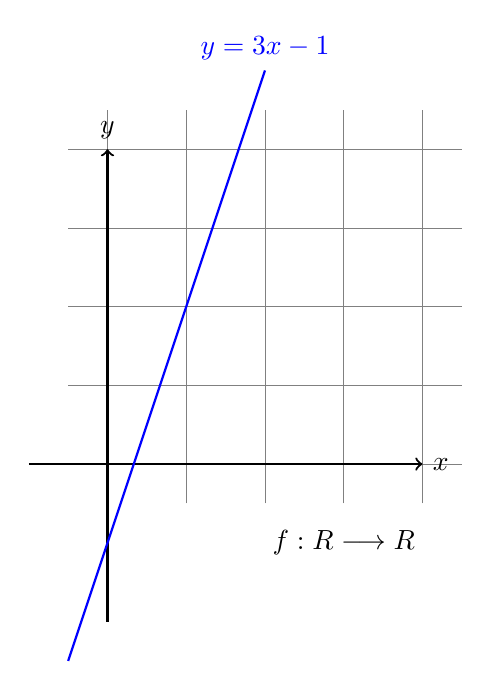
\begin{tikzpicture}
        % Disegna la griglia
        \draw[very thin, gray] (-0.5,-0.5) grid (4.5,4.5);
        
        % Disegna assi
        \draw[thick,->] (-1,0) -- (4,0) node[right] {$x$}; % Asse x
        \draw[thick,->] (0,-2) -- (0,4) node[above] {$y$}; % Asse y

        % Disegna la funzione y = 3x - 2
        \draw[domain=-0.5:2,smooth,variable=\x,blue,thick] 
        plot ({\x},{3*\x-1}) node[above] {$y = 3x - 1$};

        \node at (3, -1) {$f:\mathbb{R}\longrightarrow \mathbb{R}$};
    \end{tikzpicture} \hspace{2cm}
    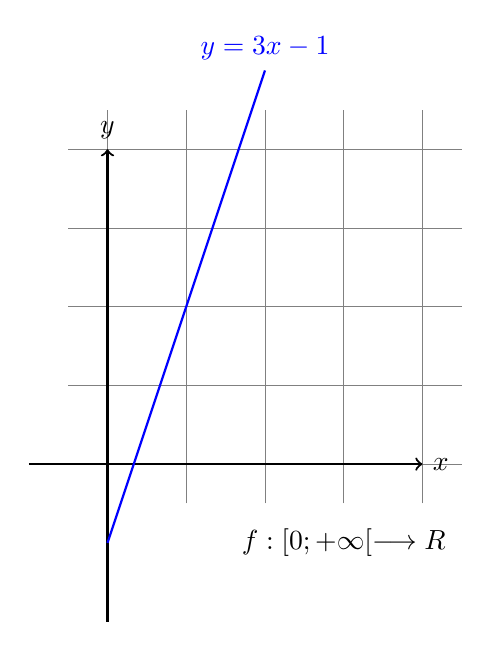
\begin{tikzpicture}
        % Disegna la griglia
        \draw[very thin, gray] (-0.5,-0.5) grid (4.5,4.5);
        
        % Disegna assi
        \draw[thick,->] (-1,0) -- (4,0) node[right] {$x$}; % Asse x
        \draw[thick,->] (0,-2) -- (0,4) node[above] {$y$}; % Asse y

        % Disegna la funzione y = 3x - 2
        \draw[domain=0:2,smooth,variable=\x,blue,thick] 
        plot ({\x},{3*\x-1}) node[above] {$y = 3x - 1$};

        \node at (3, -1) {$f:\lbrack 0; +\infty \lbrack \longrightarrow \mathbb{R}$};
    \end{tikzpicture}
\end{center}

\pagebreak
\subsection{Insieme immagini}
Sia $f:A \rightarrow B$ una funzione. Il suo insieme delle immagini è definito come segue:
$$
    Im(f)= \{ y=f(x)|x \in A \}
$$
Generalmente $x$ indica gli argomenti e $y$ le immagini, nello schema visto nell'introduzione $B$
rappresenta l'insieme delle immagini. Tutti gli elementi di $A$ sono associati ad un elemento di $B$,
ma non per forza viceversa.

\subsubsection{Esempi}
\begin{align*}
    f: \mathbb{R}& \longrightarrow \mathbb{R} \\
    x& \longmapsto y=3x-1 \\
    &\Rightarrow Im(f)=\mathbb{R}
\end{align*}
In questo caso per trovare $Im$ guardiamo il grafico.

\begin{center}
    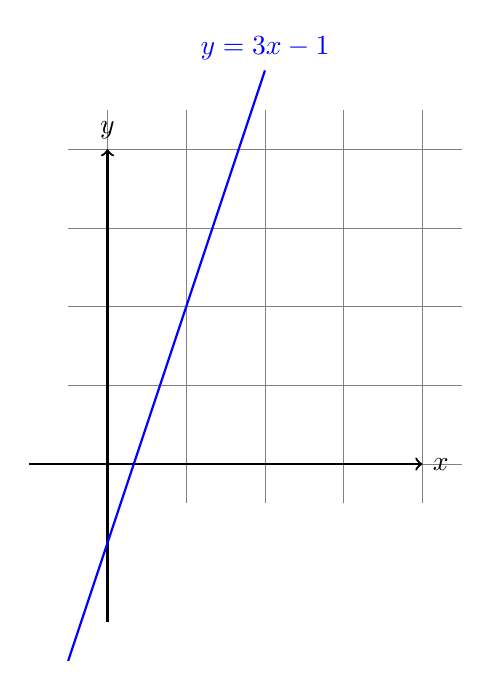
\begin{tikzpicture}
        % Disegna la griglia
        \draw[very thin, gray] (-0.5,-0.5) grid (4.5,4.5);
        
        % Disegna assi
        \draw[thick,->] (-1,0) -- (4,0) node[right] {$x$}; % Asse x
        \draw[thick,->] (0,-2) -- (0,4) node[above] {$y$}; % Asse y

        % Disegna la funzione y = 3x - 2
        \draw[domain=-0.5:2,smooth,variable=\x,blue,thick] 
        plot ({\x},{3*\x-1}) node[above] {$y = 3x - 1$};
    \end{tikzpicture}
\end{center}

\begin{align*}
    g: \mathbb{R}& \longrightarrow \mathbb{R} \\
    x& \longmapsto x^2-2 \\
    &\Rightarrow Im(g)= \lbrack -2; + \infty \lbrack \\
    &= \lbrack y_v;+ \infty \lbrack
\end{align*}
In questo caso trattandosi di una \textbf{parabola}, per determinare $Im(g)$ guardiamo il vertice.

\textbf{Nota:} Non esiste una ricetta o una procedura precisa per trovare l'$Im$ di una funzione, non è come per il dominio.

\pagebreak
\subsection{Grafico di una funzione}
Sia $f:A \rightarrow B$ una funzione. Il suo grafico $G(f)$ è l'insieme dei punti 
$$
    G(f)= \{ (a;f(a)) | a \in A \}
$$

\begin{tikzpicture}[x=0.75pt,y=0.75pt,yscale=-1,xscale=1]
    %uncomment if require: \path (0,300); %set diagram left start at 0, and has height of 300
    
    %Shape: Axis 2D [id:dp7439597163468655] 
    \draw  (60.68,251.63) -- (555.67,251.63)(110.17,137.25) -- (110.17,264.34) (548.67,246.63) -- (555.67,251.63) -- (548.67,256.63) (105.17,144.25) -- (110.17,137.25) -- (115.17,144.25)  ;
    %Straight Lines [id:da7977119812178095] 
    \draw [color={rgb, 255:red, 251; green, 0; blue, 0 }  ,draw opacity=1 ][line width=0.75]  [dash pattern={on 0.84pt off 2.51pt}]  (329.55,156.86) -- (329.83,252) ;
    %Straight Lines [id:da6782457373660774] 
    \draw [color={rgb, 255:red, 251; green, 0; blue, 0 }  ,draw opacity=1 ][line width=0.75]  [dash pattern={on 0.84pt off 2.51pt}]  (329.55,156.86) -- (313.94,156.78) -- (110,156.25) ;
    %Shape: Ellipse [id:dp1285941766712374] 
    \draw  [color={rgb, 255:red, 247; green, 2; blue, 2 }  ,draw opacity=1 ][fill={rgb, 255:red, 252; green, 5; blue, 5 }  ,fill opacity=1 ] (325.11,155.34) .. controls (325.11,153.23) and (326.73,151.52) .. (328.72,151.52) .. controls (330.72,151.52) and (332.33,153.23) .. (332.33,155.34) .. controls (332.33,157.45) and (330.72,159.17) .. (328.72,159.17) .. controls (326.73,159.17) and (325.11,157.45) .. (325.11,155.34) -- cycle ;
    %Curve Lines [id:da9750121639766473] 
    \draw [color={rgb, 255:red, 74; green, 144; blue, 226 }  ,draw opacity=1 ]   (74.37,251.93) .. controls (90.56,239.78) and (141.2,201.43) .. (175.37,207.93) .. controls (209.53,214.43) and (224.7,286.38) .. (256.37,269.93) .. controls (283.63,255.77) and (299.52,165.2) .. (325.11,156.86) .. controls (329.25,155.51) and (333.63,156.31) .. (338.37,159.93) .. controls (372.37,185.93) and (391.16,255.4) .. (440.37,267.93) .. controls (489.57,280.46) and (546.79,183.04) .. (547.37,177.93) ;
    
    % Text Node
    \draw (45.98,153.1) node [anchor=north west][inner sep=0.75pt]    {$\textcolor[rgb]{0.94,0.02,0.02}{b=f}\textcolor[rgb]{0.94,0.02,0.02}{(}\textcolor[rgb]{0.94,0.02,0.02}{a}\textcolor[rgb]{0.94,0.02,0.02}{)}$};
    % Text Node
    \draw (320.91,131.24) node [anchor=north west][inner sep=0.75pt]    {$\textcolor[rgb]{0.98,0.04,0.04}{(}\textcolor[rgb]{0.98,0.04,0.04}{a;b}\textcolor[rgb]{0.98,0.04,0.04}{)}$};
    % Text Node
    \draw (325.14,253.54) node [anchor=north west][inner sep=0.75pt]    {$\textcolor[rgb]{0.95,0.02,0.02}{a}$};
\end{tikzpicture}

$(a;b) \in G(f) \Leftrightarrow b = f(a)$, Un punto appartiene al grafico se e solo se $b=f(a)$


\textbf{Osservazione:}
\begin{center}
    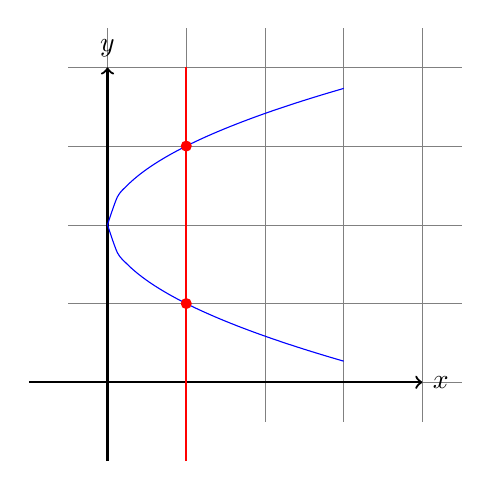
\begin{tikzpicture}
        % Disegna la griglia
        \draw[very thin, gray] (-0.5,-0.5) grid (4.5,4.5);
        
        % Disegna assi
        \draw[thick,->] (-1,0) -- (4,0) node[right] {$x$}; % Asse x
        \draw[thick,->] (0,-1) -- (0,4) node[above] {$y$}; % Asse y

        \draw[domain=0:3,smooth,variable=\x,blue] plot ({\x},{sqrt(\x) + 2});
        \draw[domain=0:3,smooth,variable=\x,blue] plot ({\x},{-sqrt(\x) + 2});

        \draw[red, thick] (1,-1) -- (1,4);  % Linea tratteggiata a x = 1

        \fill[red] (1, 1) circle (2pt);  % Punto a (1, 1) con raggio di 5pt
        \fill[red] (1, 3) circle (2pt);  % Punto a (1, 1) con raggio di 5pt
    \end{tikzpicture} \hspace{2cm}
\end{center}
Questo grafico non rappresenta una funzione, per alcuni argomenti ci sono più immagini.

\pagebreak
\subsection{Operazioni con le funzioni}
\subsubsection{Somma - Sottrazione}
Esempio:
\begin{align*}
    f(x)&=\sqrt{x+1} \Rightarrow D(f)=\lbrack-1;+\infty\lbrack \\
    g(x)&=\frac{1}{x}\Rightarrow D(g)=\mathbb{R} \backslash \{0\} \\
    (f\pm g)(x)&=\sqrt{x+1}\pm \frac{1}{x} \\
    \Rightarrow D(f+g)&=\lbrack-1;+\infty\lbrack \backslash \{0\} \\
    &=D(f)\cap D(g)
\end{align*}
\begin{center}
    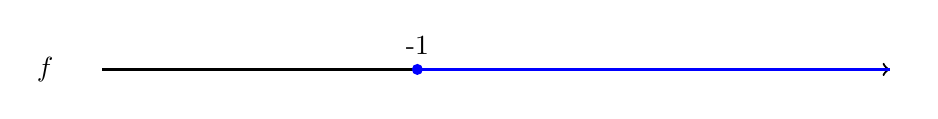
\begin{tikzpicture}        
        % Disegna assi
        \draw[thick,->] (-5,0) -- (5,0) node[right] {}; % Asse x

        \node at (-5.5, 0) {$f\phantom{+g}$};

        \node at (-1, 0.3) {-1};
        \fill[blue] (-1, 0) circle (2pt);  % Punto a (1, 1) con raggio di 5pt

        % Disegna la parte colorata in blu
        \draw[blue, thick] (-1, 0) -- (5, 0); % Parte blu della retta
    \end{tikzpicture}
\end{center}
\begin{center}
    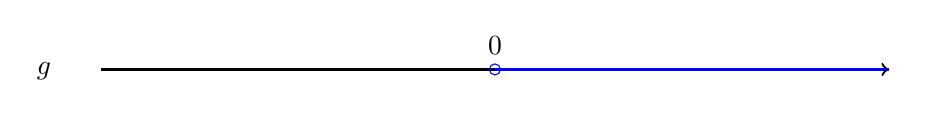
\begin{tikzpicture}        
        % Disegna assi
        \draw[thick,->] (-5,0) -- (5,0) node[right] {}; % Asse x

        \node at (-5.5, 0) {$g\phantom{+g}$};

        \node at (0, 0.3) {0};
        \draw[blue] (0, 0) circle (2pt);  % Punto a (1, 1) con raggio di 5pt

        % Disegna la parte colorata in blu
        \draw[blue, thick] (0, 0) -- (5, 0); % Parte blu della retta
    \end{tikzpicture}
\end{center}
\begin{center}
    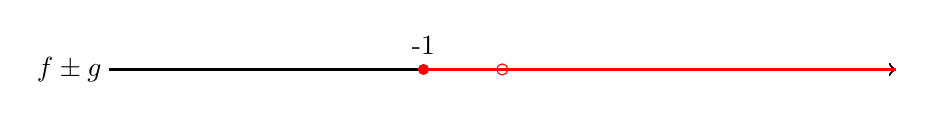
\begin{tikzpicture}        
        % Disegna assi
        \draw[thick,->] (-5,0) -- (5,0) node[right] {}; % Asse x

        \node at (-5.5, 0) {$f\pm g$};

        \node at (-1, 0.3) {-1};
        \fill[red] (-1, 0) circle (2pt);  % Punto a (1, 1) con raggio di 5pt
        \draw[red] (0, 0) circle (2pt);  % Punto a (1, 1) con raggio di 5pt

        % Disegna la parte colorata in blu
        \draw[red, thick] (-1, 0) -- (5, 0); % Parte blu della retta
    \end{tikzpicture}
\end{center}

In generale
\begin{align*}
    (f\pm g)(x) =& f(x)\pm g(x)\\
    D(f\pm g) =& D(f) \cap D(g) 
\end{align*}

\subsubsection{Prodotto}
Esempio:
\begin{align*}
    f(x) =& \sqrt{x + 1} \Rightarrow D(f) = [-1; +\infty[ \\
    g(x) =& x \Rightarrow D(g) = \mathbb{R} \\
    \Rightarrow& (f \cdot g)(x) = x \cdot \sqrt{x + 1} \\
    \Rightarrow& D(f \cdot g) = [-1;+\infty[
\end{align*}

In generale
\begin{align*}
    (f \cdot g)(x) =& f(x) \cdot g(x) \\
    D(f \cdot g) =& D(f) \cap D(g)  
\end{align*}

\subsubsection{Divisione}
Esempio:
\begin{align*}
    f(x) =& \frac{1}{x} \Rightarrow D(f) = \mathbb{R}^* \\
    g(x) =& \sqrt{x + 2} \Rightarrow D(g) = [-2;+\infty[ \\
    \Rightarrow& \frac{f}{g}(x) = \frac{1/x}{\sqrt{x + 2}} = \frac{1}{x \cdot \sqrt{x + 2}} \\
    D(\frac{f}{g}) =& \color{red}]\color{black}-2;+\infty[\backslash \{0\}
\end{align*}
\textbf{Nota:} Il dominio non è dato solo dall'intersezione, nell'esempio sopra va anche \color{red}escluso \color{black} il -2 che non si può dividere per 0.

In generale
\begin{align*}
    (\frac{f}{g})(x) =& \frac{f(x)}{g(x)} \\
    D(\frac{f}{g}) =& D(f) \cap D(g) \backslash \{x \in D(g) | g(x) = 0\}
\end{align*}

\subsubsection{Composizione di funzioni}
\begin{center}
    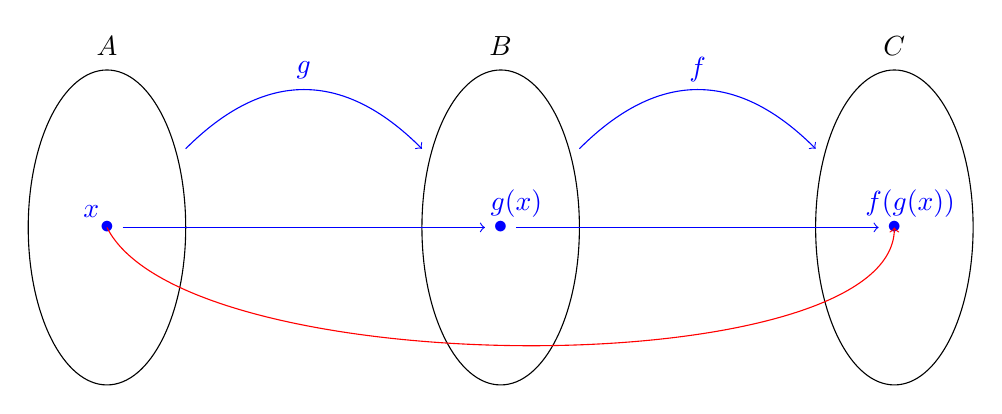
\begin{tikzpicture}
        %sets A and B
        \draw (-5,0) ellipse (1 and 2);
        \draw (0,0) ellipse (1 and 2);
        \draw (5,0) ellipse (1 and 2);
        \node at (-5, 2.3) {$A$};
        \node at (0,2.3) {$B$};
        \node at (5,2.3) {$C$};

        
        %set A
        \node at (-5,0) {\textcolor{blue}{$\bullet$}};
        \node at (-5.2, 0.2) {\textcolor{blue}{$x$}};
        
        %set B
        \node at (0,0) {\textcolor{blue}{$\bullet$}};
        \node at (0.2,0.3) {\textcolor{blue}{$g(x)$}};

        %set C
        \node at (5,0) {\textcolor{blue}{$\bullet$}};
        \node at (5.2,0.3) {\textcolor{blue}{$f(g(x))$}};
        
        %arrows
        \draw[->, blue] (-4.8,0) -- (-0.2,0);
        \draw[->, blue] (0.2,0) -- (4.8,0);

        \draw[->, blue] (-4, 1) .. controls (-3, 2) and (-2,2).. (-1, 1); % Freccia curva
        \node at (-2.5,2) {\textcolor{blue}{$g$}};
        \draw[->, blue] (1, 1) .. controls (2, 2) and (3,2).. (4, 1); % Freccia curva
        \node at (2.5,2) {\textcolor{blue}{$f$}};

        \draw[->, red] (-5, 0) .. controls (-4, -2) and (5,-2).. (5, 0); % Freccia curva
    \end{tikzpicture}
\end{center}

Esempio:
\begin{align*}
    f(x) =& \sqrt{x} \phantom{---}\Rightarrow D(f) = \lbrack 0;+\infty \lbrack \\
    g(x) =& x + 1 \phantom{---}\Rightarrow D(g) = \mathbb{R} \\
    \Rightarrow (f \circ g) (x) =& f(g(x)) = f(x+1) = \sqrt{x + 1} \\
    D(f \circ g) =& \lbrack -1; + \infty \lbrack
\end{align*}
\textbf{Nota:} Non c'è un modo per calolare il dominio senza conoscere le due funzioni, l'unico indizio che abbiamo è che
questo dominio deve essere incluso in $D(g)$.

\vspace{1cm}
In generale date due funzioni
\begin{align*}
    f: B \longrightarrow& C \\
    g: A \longrightarrow& B \\
\end{align*}
la funzione
\begin{align*}
    f \circ  g: A \longrightarrow& C \\
    x \longrightarrow& (f \circ  g)(x) = f(g(x))
\end{align*}
è detta \textbf{composizione di f con g} ($f$ composto $g$).

\textbf{Nota:} In generale $f \circ g \neq g \circ  f $, la composizione di funzioni non è commutativa. 

\pagebreak
\subsection{Funzione inversa}
Sia $f:A\rightarrow B$ una funzione

\begin{center}
    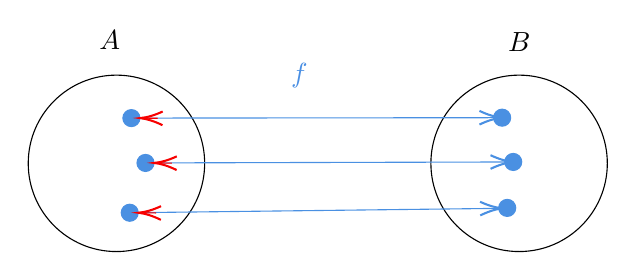
\begin{tikzpicture}[x=0.75pt,y=0.75pt,yscale=-1,xscale=1]
        %Shape: Circle [id:dp5376600122962971] 
        \draw   (147,133.5) .. controls (147,110.03) and (166.03,91) .. (189.5,91) .. controls (212.97,91) and (232,110.03) .. (232,133.5) .. controls (232,156.97) and (212.97,176) .. (189.5,176) .. controls (166.03,176) and (147,156.97) .. (147,133.5) -- cycle ;
        %Shape: Circle [id:dp22175399959501507] 
        \draw   (341,133.5) .. controls (341,110.03) and (360.03,91) .. (383.5,91) .. controls (406.97,91) and (426,110.03) .. (426,133.5) .. controls (426,156.97) and (406.97,176) .. (383.5,176) .. controls (360.03,176) and (341,156.97) .. (341,133.5) -- cycle ;
        %Shape: Circle [id:dp6720624869394561] 
        \draw  [color={rgb, 255:red, 74; green, 144; blue, 226 }  ,draw opacity=1 ][fill={rgb, 255:red, 74; green, 144; blue, 226 }  ,fill opacity=1 ] (192.6,111.7) .. controls (192.6,109.44) and (194.44,107.6) .. (196.7,107.6) .. controls (198.96,107.6) and (200.8,109.44) .. (200.8,111.7) .. controls (200.8,113.96) and (198.96,115.8) .. (196.7,115.8) .. controls (194.44,115.8) and (192.6,113.96) .. (192.6,111.7) -- cycle ;
        %Shape: Circle [id:dp7298582526690981] 
        \draw  [color={rgb, 255:red, 74; green, 144; blue, 226 }  ,draw opacity=1 ][fill={rgb, 255:red, 74; green, 144; blue, 226 }  ,fill opacity=1 ] (199.4,133.3) .. controls (199.4,131.04) and (201.24,129.2) .. (203.5,129.2) .. controls (205.76,129.2) and (207.6,131.04) .. (207.6,133.3) .. controls (207.6,135.56) and (205.76,137.4) .. (203.5,137.4) .. controls (201.24,137.4) and (199.4,135.56) .. (199.4,133.3) -- cycle ;
        %Shape: Circle [id:dp03584277532951885] 
        \draw  [color={rgb, 255:red, 74; green, 144; blue, 226 }  ,draw opacity=1 ][fill={rgb, 255:red, 74; green, 144; blue, 226 }  ,fill opacity=1 ] (191.8,157.3) .. controls (191.8,155.04) and (193.64,153.2) .. (195.9,153.2) .. controls (198.16,153.2) and (200,155.04) .. (200,157.3) .. controls (200,159.56) and (198.16,161.4) .. (195.9,161.4) .. controls (193.64,161.4) and (191.8,159.56) .. (191.8,157.3) -- cycle ;
        %Shape: Circle [id:dp2968954021217979] 
        \draw  [color={rgb, 255:red, 74; green, 144; blue, 226 }  ,draw opacity=1 ][fill={rgb, 255:red, 74; green, 144; blue, 226 }  ,fill opacity=1 ] (371.23,111.5) .. controls (371.23,109.24) and (373.07,107.4) .. (375.33,107.4) .. controls (377.6,107.4) and (379.43,109.24) .. (379.43,111.5) .. controls (379.43,113.76) and (377.6,115.6) .. (375.33,115.6) .. controls (373.07,115.6) and (371.23,113.76) .. (371.23,111.5) -- cycle ;
        %Shape: Circle [id:dp5146834779662781] 
        \draw  [color={rgb, 255:red, 74; green, 144; blue, 226 }  ,draw opacity=1 ][fill={rgb, 255:red, 74; green, 144; blue, 226 }  ,fill opacity=1 ] (376.57,132.83) .. controls (376.57,130.57) and (378.4,128.73) .. (380.67,128.73) .. controls (382.93,128.73) and (384.77,130.57) .. (384.77,132.83) .. controls (384.77,135.1) and (382.93,136.93) .. (380.67,136.93) .. controls (378.4,136.93) and (376.57,135.1) .. (376.57,132.83) -- cycle ;
        %Shape: Circle [id:dp8874180520381186] 
        \draw  [color={rgb, 255:red, 74; green, 144; blue, 226 }  ,draw opacity=1 ][fill={rgb, 255:red, 74; green, 144; blue, 226 }  ,fill opacity=1 ] (373.67,154.97) .. controls (373.67,152.7) and (375.5,150.87) .. (377.77,150.87) .. controls (380.03,150.87) and (381.87,152.7) .. (381.87,154.97) .. controls (381.87,157.23) and (380.03,159.07) .. (377.77,159.07) .. controls (375.5,159.07) and (373.67,157.23) .. (373.67,154.97) -- cycle ;
        %Straight Lines [id:da9335812660878691] 
        \draw [color={rgb, 255:red, 74; green, 144; blue, 226 }  ,draw opacity=1 ]   (196.7,111.7) -- (373.33,111.5) ;
        \draw [shift={(375.33,111.5)}, rotate = 179.94] [color={rgb, 255:red, 74; green, 144; blue, 226 }  ,draw opacity=1 ][line width=0.75]    (10.93,-3.29) .. controls (6.95,-1.4) and (3.31,-0.3) .. (0,0) .. controls (3.31,0.3) and (6.95,1.4) .. (10.93,3.29)   ;
        %Straight Lines [id:da7098845497750764] 
        \draw [color={rgb, 255:red, 74; green, 144; blue, 226 }  ,draw opacity=1 ]   (203.5,133.3) -- (378.67,132.84) ;
        \draw [shift={(380.67,132.83)}, rotate = 179.85] [color={rgb, 255:red, 74; green, 144; blue, 226 }  ,draw opacity=1 ][line width=0.75]    (10.93,-3.29) .. controls (6.95,-1.4) and (3.31,-0.3) .. (0,0) .. controls (3.31,0.3) and (6.95,1.4) .. (10.93,3.29)   ;
        %Straight Lines [id:da3061476378008071] 
        \draw [color={rgb, 255:red, 74; green, 144; blue, 226 }  ,draw opacity=1 ]   (195.9,157.3) -- (373.67,155.19) ;
        \draw [shift={(375.67,155.17)}, rotate = 179.32] [color={rgb, 255:red, 74; green, 144; blue, 226 }  ,draw opacity=1 ][line width=0.75]    (10.93,-3.29) .. controls (6.95,-1.4) and (3.31,-0.3) .. (0,0) .. controls (3.31,0.3) and (6.95,1.4) .. (10.93,3.29)   ;
        %Straight Lines [id:da5339749354113461] 
        \draw [color={rgb, 255:red, 247; green, 0; blue, 0 }  ,draw opacity=1 ]   (208.6,157.4) -- (202,157.32) ;
        \draw [shift={(200,157.3)}, rotate = 0.67] [color={rgb, 255:red, 247; green, 0; blue, 0 }  ,draw opacity=1 ][line width=0.75]    (10.93,-3.29) .. controls (6.95,-1.4) and (3.31,-0.3) .. (0,0) .. controls (3.31,0.3) and (6.95,1.4) .. (10.93,3.29)   ;
        %Straight Lines [id:da3794427356884975] 
        \draw [color={rgb, 255:red, 247; green, 0; blue, 0 }  ,draw opacity=1 ]   (216.2,133.4) -- (209.6,133.32) ;
        \draw [shift={(207.6,133.3)}, rotate = 0.67] [color={rgb, 255:red, 247; green, 0; blue, 0 }  ,draw opacity=1 ][line width=0.75]    (10.93,-3.29) .. controls (6.95,-1.4) and (3.31,-0.3) .. (0,0) .. controls (3.31,0.3) and (6.95,1.4) .. (10.93,3.29)   ;
        %Straight Lines [id:da7606811163067712] 
        \draw [color={rgb, 255:red, 247; green, 0; blue, 0 }  ,draw opacity=1 ]   (209.4,111.8) -- (202.8,111.72) ;
        \draw [shift={(200.8,111.7)}, rotate = 0.67] [color={rgb, 255:red, 247; green, 0; blue, 0 }  ,draw opacity=1 ][line width=0.75]    (10.93,-3.29) .. controls (6.95,-1.4) and (3.31,-0.3) .. (0,0) .. controls (3.31,0.3) and (6.95,1.4) .. (10.93,3.29)   ;
        
        % Text Node
        \draw (180,68.4) node [anchor=north west][inner sep=0.75pt]    {$A$};
        % Text Node
        \draw (377,69.4) node [anchor=north west][inner sep=0.75pt]    {$B$};
        % Text Node
        \draw (272.4,83.8) node [anchor=north west][inner sep=0.75pt]    {$\textcolor[rgb]{0.29,0.56,0.89}{f}$};
    \end{tikzpicture}
\end{center}
Ci chiediamo se esiste una funzione $g: B\longrightarrow A$ che fa "il contrario" di $f$, in questo caso $g$ è detta \textbf{funzione inversa}
di $f$.

\subsubsection{Definizioni}
\begin{itemize}
    \item Una funzione $f: A \longrightarrow B$ è detta \textbf{iniettiva} se \begin{align*}
        f(x_1) \neq f(x_2) \forall x_1 \neq x_2 \in A
    \end{align*}
    \textbf{Nota:} una funzione può sempre essere resa iniettiva restringendo l'insieme di partenza.
    \begin{center}
        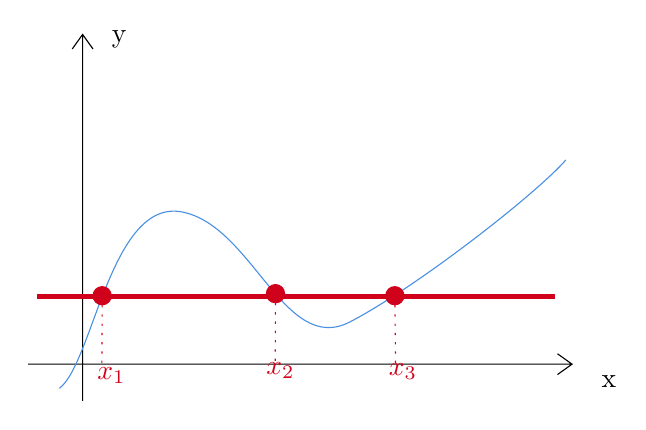
\begin{tikzpicture}[x=0.75pt,y=0.75pt,yscale=-1,xscale=1]
            %Shape: Axis 2D [id:dp9877030578675837] 
            \draw  (145,222.85) -- (407,222.85)(171.2,64) -- (171.2,240.5) (400,217.85) -- (407,222.85) -- (400,227.85) (166.2,71) -- (171.2,64) -- (176.2,71)  ;
            %Curve Lines [id:da47558611259817984] 
            \draw [color={rgb, 255:red, 74; green, 144; blue, 226 }  ,draw opacity=1 ]   (160,234.5) .. controls (176.2,222.35) and (184.83,143) .. (219,149.5) .. controls (253.17,156) and (268.33,218.95) .. (300,202.5) .. controls (331.67,186.05) and (389,141.5) .. (404,124.5) ;
            %Straight Lines [id:da941620626249894] 
            \draw [color={rgb, 255:red, 208; green, 2; blue, 27 }  ,draw opacity=1 ][line width=1.5]    (149,190.25) -- (399,190.25) ;
            %Shape: Circle [id:dp8874746484924865] 
            \draw  [color={rgb, 255:red, 208; green, 2; blue, 27 }  ,draw opacity=1 ][fill={rgb, 255:red, 208; green, 2; blue, 27 }  ,fill opacity=1 ] (317.25,189.88) .. controls (317.25,187.46) and (319.21,185.5) .. (321.63,185.5) .. controls (324.04,185.5) and (326,187.46) .. (326,189.88) .. controls (326,192.29) and (324.04,194.25) .. (321.63,194.25) .. controls (319.21,194.25) and (317.25,192.29) .. (317.25,189.88) -- cycle ;
            %Shape: Circle [id:dp7262689239269485] 
            \draw  [color={rgb, 255:red, 208; green, 2; blue, 27 }  ,draw opacity=1 ][fill={rgb, 255:red, 208; green, 2; blue, 27 }  ,fill opacity=1 ] (259.75,188.88) .. controls (259.75,186.46) and (261.71,184.5) .. (264.13,184.5) .. controls (266.54,184.5) and (268.5,186.46) .. (268.5,188.88) .. controls (268.5,191.29) and (266.54,193.25) .. (264.13,193.25) .. controls (261.71,193.25) and (259.75,191.29) .. (259.75,188.88) -- cycle ;
            %Shape: Circle [id:dp12512906493941067] 
            \draw  [color={rgb, 255:red, 208; green, 2; blue, 27 }  ,draw opacity=1 ][fill={rgb, 255:red, 208; green, 2; blue, 27 }  ,fill opacity=1 ] (176.25,189.88) .. controls (176.25,187.46) and (178.21,185.5) .. (180.63,185.5) .. controls (183.04,185.5) and (185,187.46) .. (185,189.88) .. controls (185,192.29) and (183.04,194.25) .. (180.63,194.25) .. controls (178.21,194.25) and (176.25,192.29) .. (176.25,189.88) -- cycle ;
            %Straight Lines [id:da44760789867963535] 
            \draw [color={rgb, 255:red, 208; green, 2; blue, 27 }  ,draw opacity=1 ] [dash pattern={on 0.84pt off 2.51pt}]  (180.63,189.88) -- (180.5,223.25) ;
            %Straight Lines [id:da39957355235547964] 
            \draw [color={rgb, 255:red, 208; green, 2; blue, 27 }  ,draw opacity=1 ] [dash pattern={on 0.84pt off 2.51pt}]  (264.13,188.88) -- (264,222.75) ;
            %Straight Lines [id:da8739184311558367] 
            \draw [color={rgb, 255:red, 208; green, 2; blue, 27 }  ,draw opacity=1 ] [dash pattern={on 0.84pt off 2.51pt}]  (321.63,189.88) -- (322,224.25) ;
            
            % Text Node
            \draw (420,227) node [anchor=north west][inner sep=0.75pt]   [align=left] {x};
            % Text Node
            \draw (184,61) node [anchor=north west][inner sep=0.75pt]   [align=left] {y};
            % Text Node
            \draw (177,223.4) node [anchor=north west][inner sep=0.75pt]    {$\textcolor[rgb]{0.82,0.01,0.11}{x_{1}}$};
            % Text Node
            \draw (258.5,220.9) node [anchor=north west][inner sep=0.75pt]    {$\textcolor[rgb]{0.82,0.01,0.11}{x}\textcolor[rgb]{0.82,0.01,0.11}{_{2}}$};
            % Text Node
            \draw (317.5,221.4) node [anchor=north west][inner sep=0.75pt]    {$\textcolor[rgb]{0.82,0.01,0.11}{x}\textcolor[rgb]{0.82,0.01,0.11}{_{3}}$};
        \end{tikzpicture}    

        $f(x_1) = f(x_2) = f(x_3)$, questa funzione \textbf{non} è iniettiva.   
    \end{center}
    \textbf{Nota:} una funzione è iniettiva se il suo grafico tocca al massimo ina volta qualsiasi retta orizzontale, altrimenti significa
    che elementi diversi di $A$ hanno la stessa immagine in $B$.
    \item Una funzione $f: A \longrightarrow B$ è detta \textbf{suriettiva} se \begin{align*}
        B = Im(f)
    \end{align*}
    \textbf{Nota:} una funzione può sempre essere resa usriettiva restringendo l'insieme d'arrivo dell'insieme immagini.
    \begin{center}
        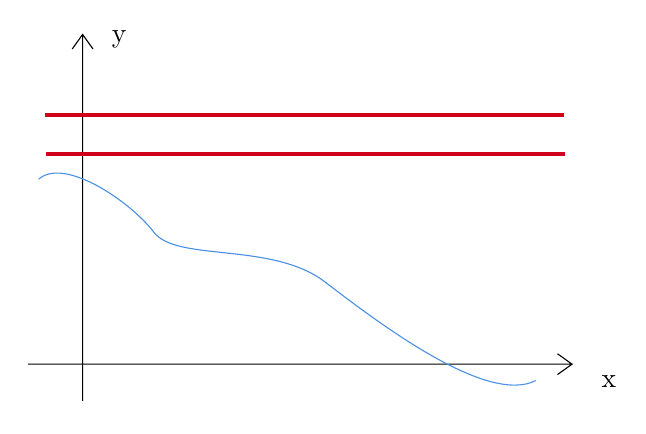
\begin{tikzpicture}[x=0.75pt,y=0.75pt,yscale=-1,xscale=1]
            %Shape: Axis 2D [id:dp7635479049905216] 
            \draw  (146,211.85) -- (408,211.85)(172.2,53) -- (172.2,229.5) (401,206.85) -- (408,211.85) -- (401,216.85) (167.2,60) -- (172.2,53) -- (177.2,60)  ;
            %Curve Lines [id:da9457720656479465] 
            \draw [color={rgb, 255:red, 74; green, 144; blue, 226 }  ,draw opacity=1 ]   (151,122.75) .. controls (163.5,111.75) and (195.5,133.75) .. (206.5,148.25) .. controls (217.5,162.75) and (263.5,152.75) .. (289,172.25) .. controls (314.5,191.75) and (367,231.75) .. (390.5,219.75) ;
            %Straight Lines [id:da2430459680033903] 
            \draw [color={rgb, 255:red, 208; green, 2; blue, 27 }  ,draw opacity=1 ][line width=1.5]    (154,91.75) -- (404,91.75) ;
            %Straight Lines [id:da22676289344682976] 
            \draw [color={rgb, 255:red, 208; green, 2; blue, 27 }  ,draw opacity=1 ][line width=1.5]    (154.5,110.75) -- (404.5,110.75) ;
            
            % Text Node
            \draw (421,216) node [anchor=north west][inner sep=0.75pt]   [align=left] {x};
            % Text Node
            \draw (185,50) node [anchor=north west][inner sep=0.75pt]   [align=left] {y};
        \end{tikzpicture}

        Ci sono delle $y$ non definite, questa funzione \textbf{non} è iniettiva         
    \end{center}
    \pagebreak
    \item Una funzione $f: A \longrightarrow B$ è detta \textbf{biettiva} se è sia iniettiva che suriettiva. In questo caso possiamo definire
    $g: B \longrightarrow A$ come segue: \begin{align*}
        g(x) = y \Leftrightarrow f(y) = x
    \end{align*}
    \begin{center}
        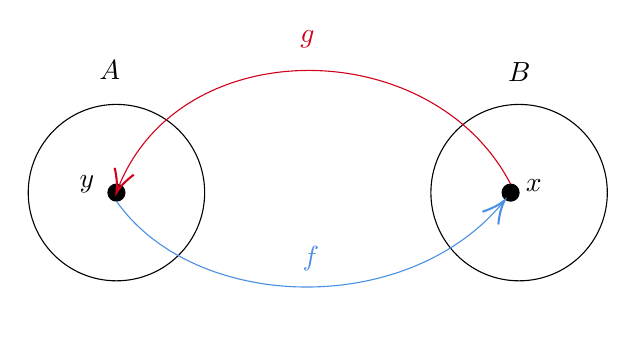
\begin{tikzpicture}[x=0.75pt,y=0.75pt,yscale=-1,xscale=1]
            %Shape: Circle [id:dp4875134192971293] 
            \draw   (136,145) .. controls (136,121.53) and (155.03,102.5) .. (178.5,102.5) .. controls (201.97,102.5) and (221,121.53) .. (221,145) .. controls (221,168.47) and (201.97,187.5) .. (178.5,187.5) .. controls (155.03,187.5) and (136,168.47) .. (136,145) -- cycle ;
            %Shape: Circle [id:dp7115025808977136] 
            \draw   (330,145) .. controls (330,121.53) and (349.03,102.5) .. (372.5,102.5) .. controls (395.97,102.5) and (415,121.53) .. (415,145) .. controls (415,168.47) and (395.97,187.5) .. (372.5,187.5) .. controls (349.03,187.5) and (330,168.47) .. (330,145) -- cycle ;
            %Shape: Circle [id:dp9300890281260831] 
            \draw  [color={rgb, 255:red, 0; green, 0; blue, 0 }  ,draw opacity=1 ][fill={rgb, 255:red, 0; green, 0; blue, 0 }  ,fill opacity=1 ] (174.4,145) .. controls (174.4,142.74) and (176.24,140.9) .. (178.5,140.9) .. controls (180.76,140.9) and (182.6,142.74) .. (182.6,145) .. controls (182.6,147.26) and (180.76,149.1) .. (178.5,149.1) .. controls (176.24,149.1) and (174.4,147.26) .. (174.4,145) -- cycle ;
            %Shape: Circle [id:dp6637339529721102] 
            \draw  [color={rgb, 255:red, 0; green, 0; blue, 0 }  ,draw opacity=1 ][fill={rgb, 255:red, 0; green, 0; blue, 0 }  ,fill opacity=1 ] (364.3,145) .. controls (364.3,142.74) and (366.14,140.9) .. (368.4,140.9) .. controls (370.66,140.9) and (372.5,142.74) .. (372.5,145) .. controls (372.5,147.26) and (370.66,149.1) .. (368.4,149.1) .. controls (366.14,149.1) and (364.3,147.26) .. (364.3,145) -- cycle ;
            %Curve Lines [id:da11912716200978934] 
            \draw [color={rgb, 255:red, 74; green, 144; blue, 226 }  ,draw opacity=1 ]   (178.5,149.1) .. controls (215.81,202.48) and (318.57,205.87) .. (364.81,149.6) ;
            \draw [shift={(365.5,148.75)}, rotate = 128.77] [color={rgb, 255:red, 74; green, 144; blue, 226 }  ,draw opacity=1 ][line width=0.75]    (10.93,-4.9) .. controls (6.95,-2.3) and (3.31,-0.67) .. (0,0) .. controls (3.31,0.67) and (6.95,2.3) .. (10.93,4.9)   ;
            %Curve Lines [id:da7677510510662031] 
            \draw [color={rgb, 255:red, 208; green, 2; blue, 27 }  ,draw opacity=1 ]   (368.4,140.9) .. controls (330.69,68.02) and (208.13,66.76) .. (178.93,143.83) ;
            \draw [shift={(178.5,145)}, rotate = 289.95] [color={rgb, 255:red, 208; green, 2; blue, 27 }  ,draw opacity=1 ][line width=0.75]    (10.93,-4.9) .. controls (6.95,-2.3) and (3.31,-0.67) .. (0,0) .. controls (3.31,0.67) and (6.95,2.3) .. (10.93,4.9)   ;
            
            % Text Node
            \draw (169,79.9) node [anchor=north west][inner sep=0.75pt]    {$A$};
            % Text Node
            \draw (366,80.9) node [anchor=north west][inner sep=0.75pt]    {$B$};
            % Text Node
            \draw (266.9,169.8) node [anchor=north west][inner sep=0.75pt]    {$\textcolor[rgb]{0.29,0.56,0.89}{f}$};
            % Text Node
            \draw (265.9,65.8) node [anchor=north west][inner sep=0.75pt]    {$\textcolor[rgb]{0.82,0.01,0.11}{g}$};
            % Text Node
            \draw (159.5,135.4) node [anchor=north west][inner sep=0.75pt]    {$y$};
            % Text Node
            \draw (374.5,137.4) node [anchor=north west][inner sep=0.75pt]    {$x$};
        \end{tikzpicture}            
    \end{center}
\end{itemize}

\vspace{1.5cm}
La funzione
\begin{align*}
    id: \mathbb{R}\longrightarrow &\mathbb{R} \\
    x \longmapsto& id(x) = x
\end{align*}
è detta \textbf{funzione identità} ed è l'elemento neutro della composizione di funzioni.

\textbf{Nota:}
\begin{align*}
    (f \circ id)(x) =& f(id(x)) = f(x) \\
    (id \circ f)(x) =& id(f(x)) = f(x)
\end{align*}

Sia $f:A\longrightarrow B$ una funzione. Se esiste una funzione $g:B\longrightarrow A$ tale che $f \circ g = id$ e $g \circ f = id$
allora $g$ è detta \textbf{inversa} di $f$ e scriviamo $g = f^{-1}$.

\subsubsection{Proprietà}
Il dominio di una funzione diventa l'insieme immagini della sua funzione inversa, viceversa l'insieme delle immagini di una funzione
diventa il dominio della sua funzione inversa:
\begin{align*}
    f:D(f)\longrightarrow& Im(f) \\
    f^{-1}:Im(f) \longrightarrow& D(f)
\end{align*}
e quindi
\begin{align*}
    D(f^{-1}) =& Im(f) \\
    Im(f^{-1}) =& D(f)
\end{align*}

Alcune proprietà sulla composizione di funzioni e sulla funzione inversa:
\begin{itemize}
    \item $f \circ g \neq g \circ f$
    \item $(f \circ g) \circ h = f \circ (g \circ h)$
    \item $f \circ f^{-1} = id$, $f^{-1} \circ f = id$
    \item $(f \circ g)^{-1} = f^{-1} \circ g^{-1}$
\end{itemize}

\pagebreak
\subsection{Funzioni elementari}
\subsubsection{La funzione affine}
Una funzione
\begin{align*}
    f: \mathbb{R} \longrightarrow& \mathbb{R} \\
    x \longmapsto& y = mx + q
\end{align*}
è detta funzione affine.
\begin{figure}[h]
    \centering
    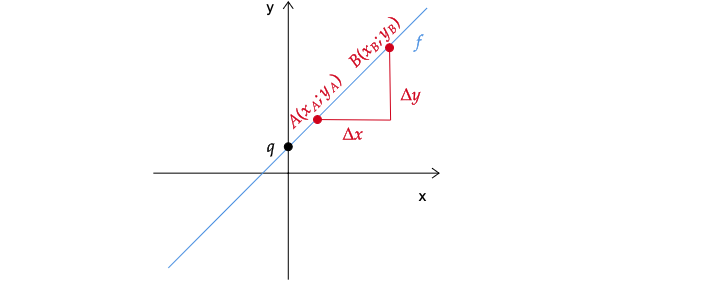
\includegraphics[width=1\textwidth]{images/funzioneLineare.png}
\end{figure}

\begin{itemize}
    \item $m$ è detta pendenza (o coefficiente angolare)
    \begin{itemize}
        \item $m = \frac{\Delta y}{\Delta x} = \frac{y_B - y_A}{x_B-x_A}$
        \item Determina la pendenza se $m>0$ sarà positiva, se $m<0$ sarà negativa
    \end{itemize}
    \item $q$ è detta ordinata all'origine ($f(0) = q$)
    \begin{itemize}
        \item Se $q = 0$, $f$ è detta funzione lineare
    \end{itemize}
    \item $D(f) = \mathbb{R}$
    \item $Im(f) = \mathbb{R}$, se $m\neq 0$
    \item $Im(f) = \{ q\} $, se $m=0$
\end{itemize}

\vspace{1.5cm}
Intersezioni con gli assi:
\begin{itemize}
    \item $\cap$ asse $y$: $(0; q)$
    \item $\cap$ asse $x$(zeri): $y = 0 \phantom{--}mx+q = 0$
    \begin{itemize}
        \item \textbf{Caso 1:} $m \neq 0 \phantom{--}x = -\frac{q}{m}$, un solo zero $(-\frac{q}{m};0)$
        \item \textbf{Caso 2:} $m = 0$ e $q \neq 0 \phantom{--} 0 \cdot x = -q$, nessuno zero
        \item \textbf{Caso 3:} $m = 0$ e $q = 0 \phantom{--} 0 \cdot x = 0$, ogni punto $(x;0), x\in\mathbb{R}$ è uno zero
    \end{itemize}
\end{itemize}

Condizioni di parallelismo e perpendicolarità:
\begin{itemize}
    \item Due rette di funzione affine sono parallele ($f/ / g$) se e solo se $m_f = m_g$
    \item Sono invece perpendicolari ($f\perp g$) se e solo se $m_f \cdot m_g = -1$ e quindi $m_g = -\frac{1}{m_f}$
\end{itemize}

\pagebreak
\subsubsection{La funzione valore assoluto}
La funzione valore assoluto è definita come segue:
\begin{align*}
    f:\mathbb{R} \longrightarrow& \mathbb{R} \\
    x \longmapsto& y = \left\lvert x\right\rvert = \begin{cases}
        -x, \phantom{-}x < 0 \\
        x, \phantom{-}x\geq 0
    \end{cases}
\end{align*}
\begin{center}
    \begin{tikzpicture}[x=0.75pt,y=0.75pt,yscale=-1,xscale=1]
        %Shape: Axis 2D [id:dp42285592065577615] 
        \draw  (210.5,189.75) -- (418,189.75)(291.5,74) -- (291.5,260.25) (411,184.75) -- (418,189.75) -- (411,194.75) (286.5,81) -- (291.5,74) -- (296.5,81)  ;
        %Straight Lines [id:da03271457993868776] 
        \draw [color={rgb, 255:red, 74; green, 144; blue, 226 }  ,draw opacity=1 ]   (398.5,81.25) -- (291.5,189.75) ;
        %Straight Lines [id:da8016276926763909] 
        \draw [color={rgb, 255:red, 74; green, 144; blue, 226 }  ,draw opacity=1 ]   (202.5,82.75) -- (291.5,189.75) ;
        %Straight Lines [id:da4748625202725838] 
        \draw [color={rgb, 255:red, 128; green, 128; blue, 128 }  ,draw opacity=1 ] [dash pattern={on 0.84pt off 2.51pt}]  (291.5,189.75) -- (264.57,213.25) -- (213,258.25) ;
        
        % Text Node
        \draw (273.5,70.5) node [anchor=north west][inner sep=0.75pt]   [align=left] {y};
        % Text Node
        \draw (401,195.5) node [anchor=north west][inner sep=0.75pt]   [align=left] {x};
        % Text Node
        \draw (354,126.4) node [anchor=north west][inner sep=0.75pt]    {$\textcolor[rgb]{0.29,0.56,0.89}{y=|x|}$};
        % Text Node
        \draw (211.5,205.4) node [anchor=north west][inner sep=0.75pt]  [color={rgb, 255:red, 128; green, 128; blue, 128 }  ,opacity=1 ]  {$\textcolor[rgb]{0.5,0.5,0.5}{y=x}$};
    \end{tikzpicture}
\end{center}

\begin{itemize}
    \item $D(f) = \mathbb{R}$
    \item $Im(f) = \mathbb{R}_+$
\end{itemize}

\pagebreak
\subsubsection{Funzioni quadratiche}
Una funzione
\begin{align*}
    f:\mathbb{R} \longrightarrow& \mathbb{R} \\
    x \longmapsto& y = ax^2 + bx + c
\end{align*}
dove $a \neq 0, b, c \in \mathbb{R}$ è detta funzione quadratica.

\begin{center}
    \begin{tikzpicture}[x=0.75pt,y=0.75pt,yscale=-1,xscale=1]
        %Shape: Axis 2D [id:dp47598527762918297] 
        \draw  (168.9,151) -- (387.9,151)(271,38.8) -- (271,219.3) (380.9,146) -- (387.9,151) -- (380.9,156) (266,45.8) -- (271,38.8) -- (276,45.8)  ;
        %Shape: Parabola [id:dp6755288498451852] 
        \draw  [color={rgb, 255:red, 74; green, 144; blue, 226 }  ,draw opacity=1 ] (241.07,65.33) .. controls (286.4,205.33) and (331.73,205.33) .. (377.07,65.33) ;
        %Shape: Circle [id:dp8949268520745572] 
        \draw  [color={rgb, 255:red, 74; green, 144; blue, 226 }  ,draw opacity=1 ][fill={rgb, 255:red, 74; green, 144; blue, 226 }  ,fill opacity=1 ] (305.9,170.33) .. controls (305.9,168.58) and (307.32,167.17) .. (309.07,167.17) .. controls (310.82,167.17) and (312.23,168.58) .. (312.23,170.33) .. controls (312.23,172.08) and (310.82,173.5) .. (309.07,173.5) .. controls (307.32,173.5) and (305.9,172.08) .. (305.9,170.33) -- cycle ;
        
        % Text Node
        \draw (375.2,156.6) node [anchor=north west][inner sep=0.75pt]   [align=left] {x};
        % Text Node
        \draw (253.2,45) node [anchor=north west][inner sep=0.75pt]   [align=left] {y};
        % Text Node
        \draw (271.67,174) node [anchor=north west][inner sep=0.75pt]   [align=left] {\textcolor[rgb]{0.29,0.56,0.89}{Vertice}};
        % Text Node
        \draw (323.67,174.07) node [anchor=north west][inner sep=0.75pt]    {$\textcolor[rgb]{0.29,0.56,0.89}{V}$};
        % Text Node
        \draw (368.67,87.73) node [anchor=north west][inner sep=0.75pt]    {$\textcolor[rgb]{0.29,0.56,0.89}{f}$};
    \end{tikzpicture}
\end{center}

\begin{itemize}
    \item $a$ definisce il "verso" della parabola, se $a>0$ sorride, se $a<0$ è triste
    \item $c$ definisce l'intersezione con l'asse $y$, $I_y = (0;c)$
    \begin{itemize}
        \item se $b=0$ corrisponde al vertice
    \end{itemize}
    \item $b$ è il punto sulla quale "ruota" la parabola
    \begin{itemize}
        \item se $c=0$ il vertice è definito come $V(x_v;f(x_v)) = (-\frac{b}{2a};f(-\frac{b}{2a}))$
    \end{itemize}
\end{itemize}

\vspace{1cm}
In generale per trovare il vertice di una parabola vale:
\begin{align*}
    V = (-\frac{b}{2a};f(-\frac{b}{2a})) = (-\frac{b}{2a}; \frac{\Delta}{4a})
\end{align*}
dove ovviamente
\begin{align*}
    \Delta = 4ac-b^2
\end{align*}

Si può inoltre dimostrare che per una parabola $f(x) = ax^2 + bx + c$ con vertice $V(x_v;y_v)$ vale
\begin{align*}
    f(x) = a(x-x_v)^2 + y_v
\end{align*}

\vspace{1cm}
Per trovare gli zeri di una parabola possiamo usare
\begin{align*}
    x_{1,2} = \frac{-b\pm \sqrt{\Delta}}{2a}
\end{align*}

Inoltre $\Delta$ determina il numero di soluzioni di una parabola:
\begin{itemize}
    \item se $\Delta > 0$ l'equazione ha due soluzioni reali distinte
    \item se $\Delta = 0$ l'equazione ha come unica soluzione il punto $x_v$ e il vertice sarà $V = (x_v;0)$
    \item se $\Delta < 0$ l'equazione non ha soluzioni in $\mathbb{R}$, la parabola non interseca l'asse $x$
\end{itemize}

Se $\Delta x \geq 0$ allora
\begin{itemize}
    \item $x_1 + x_2 = -\frac{b}{a}$
    \item $x_1 \cdot x_2 = \frac{c}{a}$
    \item $ax^2+bx+c = a(x-x_1)(x-x_2)$
\end{itemize}

\pagebreak
\subsubsection{La funzione polinomiale}
Una funzione
\begin{align*}
    f:\mathbb{R} \longrightarrow& \mathbb{R} \\
    x \longmapsto& y = c_nx^n + c_{n-1}x^{n-1} + ... + c_1x + c_0
\end{align*}
dove
\begin{align*}
    n \in \mathbb{N}, c_0,c_1, ..., c_n \in \mathbb{R}, c_n \neq 0
\end{align*}
è detta funzione polinomiale.

\textbf{Nota:} l'indice $n$ è detto \underline{grado} di $f$.

\vspace{1.5cm}
Il grafico delle funzioni polinomiali è così rappresentato:
\begin{figure}[h]
    \centering
    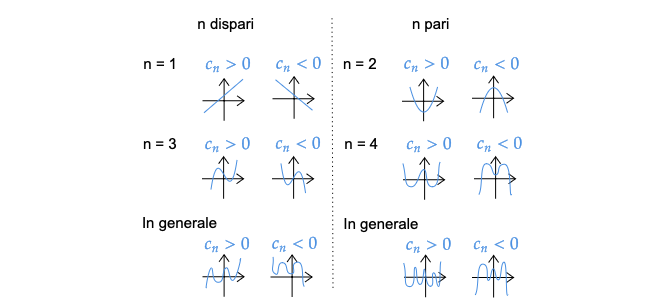
\includegraphics[width=1\textwidth]{images/funzioniPolinomiali.png}
\end{figure}

Inoltre se consideriamo ad esempio:
$$
    f(x) = (x+3)(x+1)^2(x-1)^3(x-3)^4
$$
Con zeri: $(-3;0), (-1;0), (1;0), (3;0)$

\begin{itemize}
    \item Se $(x-x_0)^n$ ha $n$ dispari la funzione \textbf{attraverserà} il punto
    \item Se $(x-x_0)^n$ ha $n$ pari la funzione \textbf{toccherà} il punto e tornerà indietro
\end{itemize}


\pagebreak
\paragraph{Operazioni con i polinomi}
\subparagraph{Somma-Differenza}

Esempi:
\begin{align*}
    &(2x^3 + 3x -2) + (3x^3 + 2x^2 -x + 3) \\
    &= 5x^3 + 2x^2 + 2x + 1
\end{align*}
\begin{align*}
    &(2x^3 + 3x -2) - (3x^3 + 2x^2 -x + 3) \\
    &= -x^3 -2x^2 + 4 x - 5 
\end{align*}
\textbf{Nota:} $grado(f\pm g) = max(grado(f);grado(g))$

\subparagraph{Prodotto}

Esempio:
\begin{align*}
    &(2x^3 + x - 1) \cdot (3x^2 -2x + 4) \\
    &= 6x^5 - 4x^4 + 8x^3 + 3x^3 - 2x^2 + 4x - 3x^2 + 2x -4 \\
    &= 6x^5 - 4x^4 + 11x^3 -5x^2 + 6x -4
\end{align*}
\textbf{Nota:} $grado(f \cdot g) = grado(f) + grado(g)$

\subparagraph{Divisione}

Esempio:
\begin{itemize}
    \item $N(x) = 14x^3 -29x^2 -5$
    \item $D(x) = 2x^2 -3x + 1$
    \item $N(x) : D(x) = ?$
\end{itemize}
\begin{figure}[h]
    \centering
    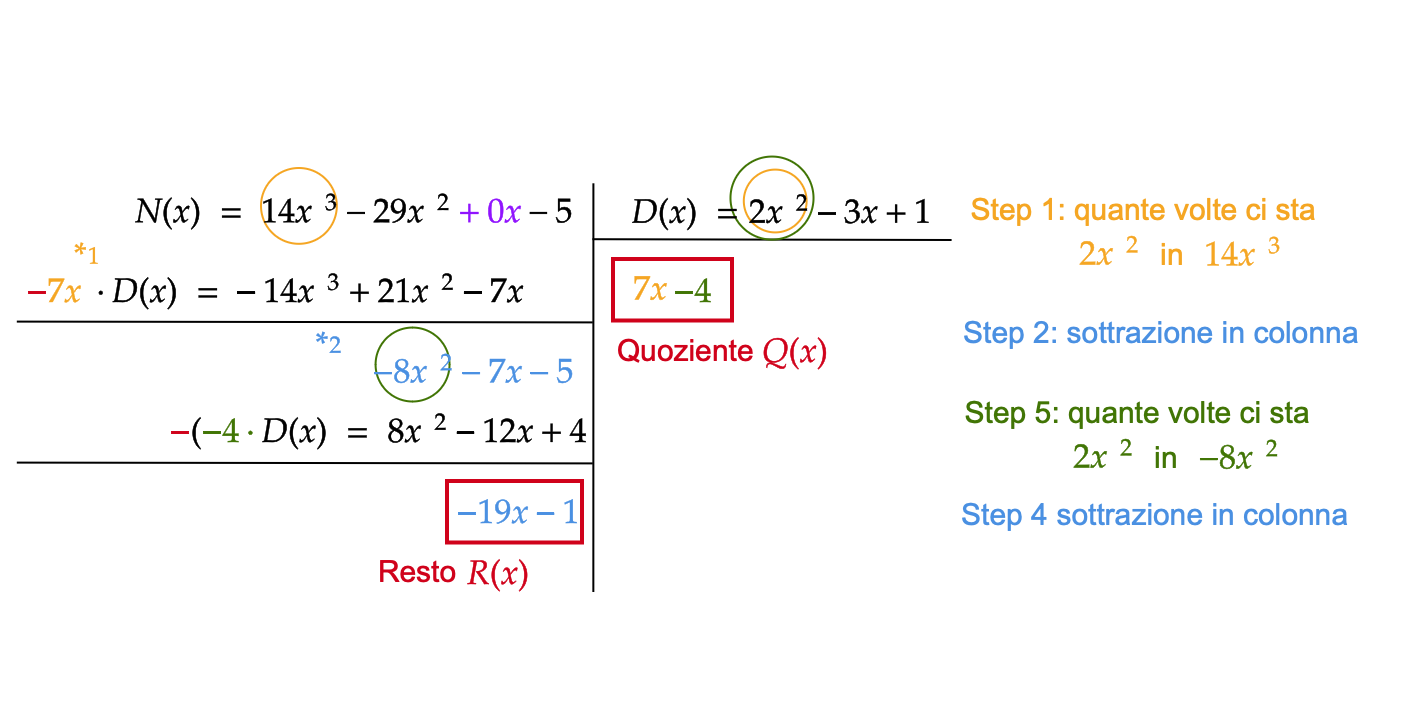
\includegraphics[width=0.8\textwidth]{images/divisionePolinomiale.png}
\end{figure}

Il risultato si scrive
$$
    N(x) = (7x-4) \cdot D(x) -19x -1
$$
oppure
$$
    \frac{N(x)}{D(x)} = 7x-4 + \frac{-19x-1}{D(x)}
$$

\pagebreak
\subsubsection{La funzione razionale fratta}
Una funzione
\begin{align*}
    f: D(f)& \longrightarrow Im(f) \\
    x& \longmapsto f(x) = \frac{N(x)}{D(x)}
\end{align*}
dove $N(x)$ e $D(x)$ sono polinomi, è detta funzione razionale fratta.

\begin{itemize}
    \item Se $grado(N(x)) < grado(D(x))$, la frazione $\frac{N(x)}{D(x)}$ è detta \textbf{propria}
    \item Se $grado(N(x)) \geq  grado(D(x))$, la frazione $\frac{N(x)}{D(x)}$ è detta \textbf{impropria} \\
    In questo caso possiamo eseguire una divisione polinomiale \\
    \textbf{Nota:} ricorda che:
    \begin{align*}
        \frac{N(x)}{D(x)} = Q(x) + \frac{R(x)}{D(x)}
    \end{align*}
\end{itemize}

\paragraph{Funzione omografica}
L'esempio più semplice di funzione razionale fratta è la funzione omografica. Una funzione
\begin{align*}
    f:D(f) \longrightarrow Im(f) \\
    x \longmapsto f(x) = \frac{ax + b}{cx + d}
\end{align*}
dove $a,b,c,d \in \mathbb{R}$ e $c \neq 0$ è detta funzione omografica. Il grafico di una funzione di questo tipo è detto \textbf{iperbole}.

\textbf{Nota:} se $c = 0 \Rightarrow f(x) = \frac{ax+b}{d} = \frac{a}{d}x + \frac{b}{d}$ (è una retta).

\pagebreak
\paragraph{In generale}
se $f(x) = \frac{ax + b}{cx + d}$
\begin{itemize}
    \item \textbf{$D(f)$:} \begin{align*}
        cx + d \neq& 0 \\
        D(f) =&\mathbb{R}\backslash \{ -\frac{d}{c}\} \\
        \Rightarrow \text{La retta } x =& -\frac{d}{c} \text{ è un asintoto verticale.}
    \end{align*} 
    \item \textbf{$Im(f)$:} \begin{align*}
        Im(f) = D(f^{-1}) = \mathbb{R}\backslash\{ \frac{a}{c}\}
    \end{align*}
    \item \textbf{$\cap$ asse $x$:} \begin{align*}
        f(x) =& 0 \\
        \frac{ax + b}{cx + d} =& 0 \\
        x =& -\frac{b}{a}
    \end{align*}
\end{itemize}
\begin{center}
    \begin{tikzpicture}[x=0.75pt,y=0.75pt,yscale=-1,xscale=1]
        %Shape: Axis 2D [id:dp005291160676745177] 
        \draw  (204.5,154.25) -- (464,154.25)(334,48) -- (334,249.75) (457,149.25) -- (464,154.25) -- (457,159.25) (329,55) -- (334,48) -- (339,55)  ;
        %Curve Lines [id:da910684277075739] 
        \draw    (207.8,206.6) .. controls (232.2,206.6) and (330.49,184.74) .. (377,146.6) .. controls (423.51,108.46) and (446.6,79.4) .. (446.2,51.4) ;
        %Shape: Circle [id:dp9993648159080415] 
        \draw  [color={rgb, 255:red, 208; green, 2; blue, 27 }  ,draw opacity=1 ][fill={rgb, 255:red, 208; green, 2; blue, 27 }  ,fill opacity=1 ] (331.4,171.5) .. controls (331.4,170.01) and (332.61,168.8) .. (334.1,168.8) .. controls (335.59,168.8) and (336.8,170.01) .. (336.8,171.5) .. controls (336.8,172.99) and (335.59,174.2) .. (334.1,174.2) .. controls (332.61,174.2) and (331.4,172.99) .. (331.4,171.5) -- cycle ;
        %Shape: Circle [id:dp2545453760323153] 
        \draw  [color={rgb, 255:red, 74; green, 144; blue, 226 }  ,draw opacity=1 ][fill={rgb, 255:red, 74; green, 144; blue, 226 }  ,fill opacity=1 ] (363.4,153.9) .. controls (363.4,152.41) and (364.61,151.2) .. (366.1,151.2) .. controls (367.59,151.2) and (368.8,152.41) .. (368.8,153.9) .. controls (368.8,155.39) and (367.59,156.6) .. (366.1,156.6) .. controls (364.61,156.6) and (363.4,155.39) .. (363.4,153.9) -- cycle ;
        %Straight Lines [id:da5180523753080537] 
        \draw [color={rgb, 255:red, 144; green, 19; blue, 254 }  ,draw opacity=1 ] [dash pattern={on 0.84pt off 2.51pt}]  (451.4,51) -- (450.2,228.2) ;
        %Straight Lines [id:da17361609678654089] 
        \draw [color={rgb, 255:red, 245; green, 166; blue, 35 }  ,draw opacity=1 ] [dash pattern={on 0.84pt off 2.51pt}]  (194.2,211.4) -- (479.8,209.8) ;
        %Shape: Circle [id:dp34142742489009315] 
        \draw  [color={rgb, 255:red, 144; green, 19; blue, 254 }  ,draw opacity=1 ][fill={rgb, 255:red, 144; green, 19; blue, 254 }  ,fill opacity=1 ] (447.4,154.7) .. controls (447.4,153.21) and (448.61,152) .. (450.1,152) .. controls (451.59,152) and (452.8,153.21) .. (452.8,154.7) .. controls (452.8,156.19) and (451.59,157.4) .. (450.1,157.4) .. controls (448.61,157.4) and (447.4,156.19) .. (447.4,154.7) -- cycle ;
        %Shape: Circle [id:dp323486964304883] 
        \draw  [color={rgb, 255:red, 245; green, 166; blue, 35 }  ,draw opacity=1 ][fill={rgb, 255:red, 245; green, 166; blue, 35 }  ,fill opacity=1 ] (331.6,210.6) .. controls (331.6,209.11) and (332.81,207.9) .. (334.3,207.9) .. controls (335.79,207.9) and (337,209.11) .. (337,210.6) .. controls (337,212.09) and (335.79,213.3) .. (334.3,213.3) .. controls (332.81,213.3) and (331.6,212.09) .. (331.6,210.6) -- cycle ;
        %Curve Lines [id:da8040145964283448] 
        \draw [color={rgb, 255:red, 74; green, 144; blue, 226 }  ,draw opacity=1 ]   (454.5,251.25) .. controls (456.5,228.25) and (445.5,212.75) .. (497,212.75) ;
        
        % Text Node
        \draw (340.4,169.2) node [anchor=north west][inner sep=0.75pt]    {$\textcolor[rgb]{0.82,0.01,0.11}{\frac{b}{d}}$};
        % Text Node
        \draw (347.2,109.6) node [anchor=north west][inner sep=0.75pt]    {$\textcolor[rgb]{0.29,0.56,0.89}{-\frac{b}{a}}$};
        % Text Node
        \draw (314.4,214.63) node [anchor=north west][inner sep=0.75pt]    {$\textcolor[rgb]{0.96,0.65,0.14}{\frac{a}{c}}$};
        % Text Node
        \draw (458.11,106.06) node [anchor=north west][inner sep=0.75pt]    {$\textcolor[rgb]{0.56,0.07,1}{-\frac{d}{c}}$};
    \end{tikzpicture}        
\end{center}

\end{document}